\documentclass[../../main.tex]{subfiles}

\graphicspath{{../../image/}{../../figure/}}

\begin{document}

\section{目标检测}\label{section:ch10-目标检测}

前面主要以图像分类问题为例介绍了 CNN 的设计动机，其中整幅图像被分类为单一类别，例如“猫”或“自行车”。这在诸如 ImageNet 的数据集上是合理的，因为每幅图像都设计为主要包含单一对象。然而，还有许多其他应用可以利用 CNN 内建的归纳偏置。更一般地说，如果 CNN 中的卷积层已经在大型图像数据集的特定任务上训练好，那么 CNN 就可以学习具有广泛适用性的内部表示。因此，我们可以针对大量的特定任务对 CNN 进行微调（参见\cref{section:ch06-深度网络}）。你已经看到了一个在 ImageNet 数据上训练好的卷积网络的例子，其通过迁移学习能够在皮肤病变图像的分类上达到人类水平（参见\cref{section:ch01-深度学习的影响}）。

图像中有多个对象属于一个或多个类别的情况很常见，我们可能希望检测其中每个对象的存在及其所属的类别。此外，在许多计算机视觉应用中，我们还需要确定在图像中检测到的任何对象的位置。例如，使用 RGB 摄像头的自动驾驶车辆可能需要检测行人的存在和位置，并识别道路标志、其他车辆等。

\subsection{边界框}\label{subsection:ch10-边界框}

考虑明确图像中对象位置的问题。一种广泛使用的方法是定义一个边界框（bounding box），它是一个紧密贴合对象边界的矩形，如\cref{figure:ch10-边界框}所示。边界框可以由其中心坐标以及宽度和高度定义，形式为向量 $\mathbf{b}=(b_x,b_y,b_w,b_h)$。这里 $\mathbf{b}$ 中的元素可以以像素为单位指定，也可以用连续数字表示。按照惯例，图像的左上角对应坐标 $(0,0)$，右下角对应坐标 $(1,1)$。

\begin{definition}[边界框]\label{definition:ch10-边界框}
称图像中一个紧密贴合对象边界的矩形为\textbf{边界框}（bounding box），并用向量 $\mathbf{b}=(b_x,b_y,b_w,b_h)$ 描述它，其中 $(b_x,b_y)$ 为框中心坐标，$b_w$ 与 $b_h$ 为宽度与高度。若采用归一化坐标，则图像左上角为 $(0,0)$、右下角为 $(1,1)$，此时 $b_x,b_y,b_w,b_h\in[0,1]$；若采用像素坐标，则各分量以像素为单位。
\end{definition}

% SUPPLEMENT: parent=definition:ch10-边界框; kind=motivation; location=紧随其后的 remark（重构新增）
\begin{remark}（重构新增）
把边界框参数化为“中心 + 宽高”而不是“左上角 + 右下角”，是为了让四个分量在尺度变换下具有统一的行为：平移只改变 $b_x,b_y$，缩放同时改变四个分量，回归时不会出现“一个角动、另一个角不动”的耦合。定义中两种坐标制的并存也有实际后果：归一化坐标使不同分辨率的图像可以共用同一套回归目标，像素坐标则便于与图像数组直接对齐；二者之间的换算是固定的线性变换，不改变框的几何。矩形“紧密贴合”只是语义要求，实际标注总会留下余量，因此预测框与真值框几乎不可能完全重合，这正是需要\cref{definition:ch10-交并比}的原因。
\end{remark}

\begin{figure}[htbp]
  \centering
  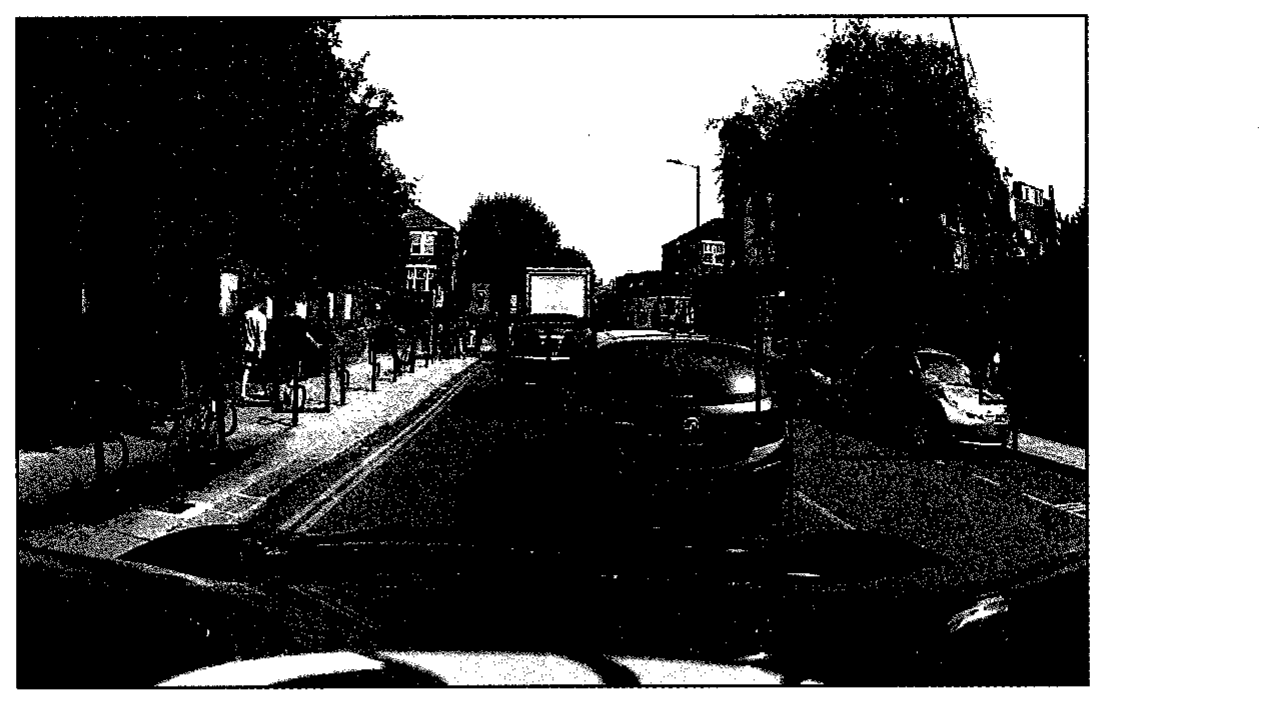
\includegraphics[width=0.72\textwidth]{ch10-fig10-19-边界框.png}
  \caption{包含不同类别的多个对象的图像，其中每个对象的位置由一个称为边界框的紧密贴合矩形标记。蓝色框对应“汽车”类别，红色框对应“行人”类别，橙色框对应“交通信号灯”类别［原始图像由 Wayve Technologies Ltd.\ 提供］。}
  \label{figure:ch10-边界框}
\end{figure}

当假设图像有且仅有一个对象，且该对象来自一个预定义的类别集合（其中的类别数量为 $C$）时，CNN 通常会有 $C$ 个输出单元，其激活函数由 softmax 函数定义（参见\cref{chapter:ch05-分类}）。对象可以由 4 个额外的具有线性激活函数的输出来定位，用于训练预测边界框坐标 $(b_x,b_y,b_w,b_h)$。由于这些量是连续的，因此可以使用对应输出的平方和误差函数。例如，Redmon et al. (2015) 使用此方法首先将图像划分成一个 $7\times 7$ 的网格；然后对于每个网格单元，使用卷积网络并基于从整个图像中提取的特征，输出与网格单元关联的任意对象的类别和边界框坐标。

\subsection{交并比}\label{subsection:ch10-交并比}

我们需要一种有意义的方式来衡量训练好的网络在预测边界框方面的性能。在图像分类中，网络的输出是类别标签的概率分布，我们可以通过查看测试集上真实类别标签的对数似然来衡量性能。然而，在对象定位中，我们需要某种方法来衡量边界框相对于某些真值的准确性，其中后者可以通过像人工标注这样的方式获得。预测框与目标框的重合程度可以用作这种度量的基础，但重叠区域的面积会取决于图像中对象的大小。此外，如果预测的边界框超出实际的边界框，则应该受到惩罚。一种能够较好地解决这两个问题的度量方法称为交并比（Intersection-over-Union, IoU），它是这两个边界框的交集区域面积与并集区域面积的比值，如\cref{figure:ch10-交并比}所示。注意，IoU 度量的取值范围是 $0\sim 1$。如果 IoU 度量超过某个阈值（通常为 $0.5$），则可以将预测标记为正确。注意，IoU 通常不直接用作训练的损失函数，因为想要通过梯度下降优化它很困难，因此通常使用中心对象来训练，而 IoU 分数主要用作评价指标。

\begin{definition}[交并比]\label{definition:ch10-交并比}
设 $B$ 与 $B'$ 是两幅同坐标系下的边界框，记 $|B|$ 为框 $B$ 所围区域的面积。称
\begin{align}
  \mathrm{IoU}(B,B')=\frac{|B\cap B'|}{|B\cup B'|}
  \label{align:ch10-交并比}
\end{align}
为 $B$ 与 $B'$ 的\textbf{交并比}（Intersection-over-Union, IoU），并约定当分母为零（两框面积均为零）时该值无定义。
\end{definition}

% SUPPLEMENT: parent=definition:ch10-交并比; kind=motivation; location=紧随其后的 remark（重构新增）
\begin{remark}（重构新增）
IoU 的设计回应了两个具体问题：用比值而不是交集面积，消除了对象大小对度量的影响（大对象天然有大交集）；用并集作分母而不是用真值框面积，使“预测框超出真值框”受到惩罚（超出部分增大并集、压低比值）。定义中“同坐标系”不能省：若一个是归一化坐标、另一个是像素坐标，比值会算出无意义的数。分母为零的退化情形必须排除，否则出现 $0/0$。IoU 不是损失函数的好选择，原因在定义之外：它是分段有理函数，在两框不相交时梯度为零，无法告诉模型“该往哪个方向移动框”，这也是实际训练常用平滑替代损失（如 $1-\mathrm{IoU}$ 的可微变体或平方和误差）而只在评价时用 IoU 的原因。
\end{remark}

\begin{figure}[htbp]
  \centering
  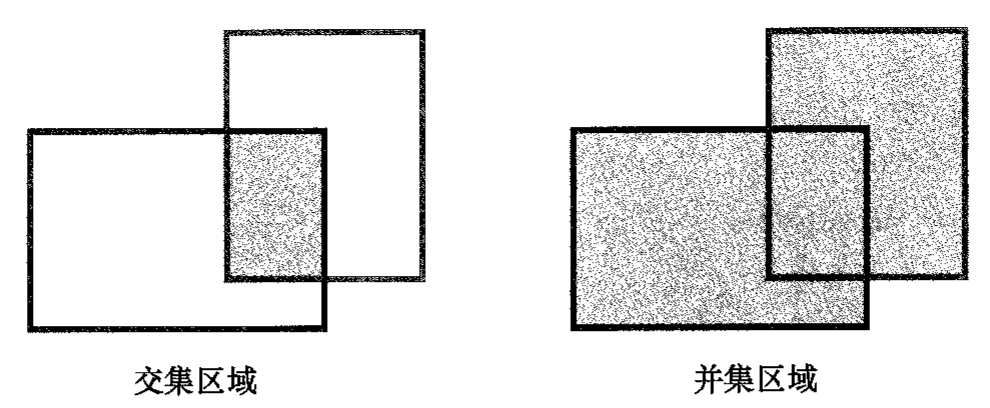
\includegraphics[width=0.72\textwidth]{ch10-fig10-20-交并比.png}
  \caption{用于量化边界框预测准确性的交并比示意图。如果预测的边界框如蓝色矩形所示，而实际的边界框如红色矩形所示，则将交并比定义为这两个框的交集区域面积（左图的绿色部分）与并集区域面积（右图的绿色部分）的比值。}
  \label{figure:ch10-交并比}
\end{figure}

\begin{proposition}[交并比的取值范围与退化情形]\label{proposition:ch10-IoU性质}
设 $B,B'$ 为面积非零的边界框。则 $0\leqslant\mathrm{IoU}(B,B')\leqslant1$，且 $\mathrm{IoU}(B,B')=1$ 当且仅当 $B=B'$（忽略零面积的边界重叠）；当 $B\cap B'$ 的内部为空时 $\mathrm{IoU}(B,B')=0$。此外，若把两框同时平移同一向量，则 IoU 不变。
\end{proposition}
\begin{proof}
由 $B\cap B'\subseteq B\cup B'$ 及面积单调性，$0\leqslant|B\cap B'|\leqslant|B\cup B'|$，而分母 $|B\cup B'|>0$，故 $0\leqslant\mathrm{IoU}\leqslant1$。若 $\mathrm{IoU}=1$，则 $|B\cap B'|=|B\cup B'|$，而 $B\cap B'\subseteq B\cup B'$，故二者至多相差一个零面积集，即 $B=B'$（忽略边界）。反之 $B=B'$ 时交集等于并集，比值为 $1$。若两框内部不相交，则 $|B\cap B'|=0$，故 IoU 为 $0$。平移不变性：设 $T$ 为平移，则 $T(B\cap B')=T(B)\cap T(B')$、$T(B\cup B')=T(B)\cup T(B')$，且平移保持面积，故比值不变。证毕。
\end{proof}

% SUPPLEMENT: parent=proposition:ch10-IoU性质; kind=motivation; location=紧随其后的 remark（重构新增）
\begin{remark}（重构新增）
这个命题给出的是 IoU 作为度量的最低要求：有界、只在完全重合时取上界、不相交时取下界、对位置平移不敏感（它只关心相对重合）。注意“当且仅当 $B=B'$”排除了仅边界接触的情形，因为边界面积为零、不影响比值，这说明 IoU 对“贴合但不重叠”和“完全分离”给出相同的分数 $0$，这是它作为评价指标的粗糙之处。平移不变性有实际用途：它说明 IoU 不依赖于对象在图像中的绝对位置，因此可以跨图像比较。命题没有说 IoU 对旋转或缩放不变，事实上矩形框在旋转下不再是矩形，定义本身就不再适用。
\end{remark}

\subsection{滑动窗口}\label{subsection:ch10-滑动窗口}

一种进行目标检测和目标定位的方法是，首先创建一个训练集，其中既包括所要检测对象的紧密裁剪的样本，也包括不包含任何对象（“背景”类别）的图像类似裁剪区域的样本。这个训练集用于训练分类器，例如一个深度 CNN，其输出表示输入窗口中存在特定对象类别的概率。然后，训练好的模型通过在图像上“扫描”输入窗口来检测新图像中的对象，并针对每个位置，将图像的结果集合用作分类器的输入。这称为滑动窗口（sliding window）。当以较高概率检测到对象时，窗口位置就是相应的边界框。

\begin{definition}[滑动窗口]\label{definition:ch10-滑动窗口}
设已用“目标窗口/背景窗口”训练好一个窗口分类器 $f$（输出窗口内存在各类对象的概率）。在图像上按固定步幅依次放置尺寸固定的输入窗口，对每个窗口计算 $f$，并把概率超过阈值的窗口位置作为检测结果，称此检测方法为\textbf{滑动窗口}（sliding window）。窗口的尺寸与步幅统称为该方法的尺度参数。
\end{definition}

% SUPPLEMENT: parent=definition:ch10-滑动窗口; kind=motivation; location=紧随其后的 remark（重构新增）
\begin{remark}（重构新增）
滑动窗口把“检测”化归为“逐窗口分类”，因此它不需要新的学习算法，只需要一个已经训练好的分类器；代价是计算：窗口位置数约为 $(J/s)\times(K/s)$，每个位置都要跑一次完整前向传播。定义中的步幅是一个显式的取舍参数：步幅小则定位精度高但计算量大，步幅大则相反。阈值则控制查全与查准的平衡。注意定义要求分类器在“背景”类上训练过，否则网络会对不含对象的窗口也给出高置信度的某一类，产生大量假阳性。后文\cref{subsection:ch10-滑动窗口}的卷积化实现之所以能大幅降低计算量，是因为它把所有这些窗口的前向传播合并成了一次卷积，而不是因为改变了定义。
\end{remark}

这种方法的一个明显缺点是，由于图像中潜在窗口位置的数量十分庞大，因此计算成本可能非常高。此外，为了适应图像中不同大小的对象，可能需要使用不同尺度的窗口重复该过程。我们可以通过在图像上以大于 1 像素的步幅在水平和垂直方向上移动输入窗口来节省计算成本。然而，使用较小步幅提高定位精度与使用较大步幅降低计算成本之间存在权衡。滑动窗口方法的计算成本对于简单分类器而言可能是合理的，但对于潜在包含数百万参数的深度神经网络来说，计算成本难以承受。

幸运的是，神经网络的卷积结构可以大大提高效率（Sermanet et al., 2013）。我们注意到，这种网络中的卷积层本身就涉及在输入图像中以跨步的方式滑动共享权重的特征检测器。因此，当使用滑动窗口通过卷积网络进行多次前向传播时，计算中存在大量冗余，如\cref{figure:ch10-滑动窗口冗余}所示。

由于滑动窗口的计算结构与卷积的计算结构相似，因此在卷积网络中高效地实现滑动窗口非常简单。考虑\cref{figure:ch10-简单卷积网络}中一个简化的卷积网络，它包括卷积层，后跟最大池化层，然后是全连接层。为简便起见，我们在每层中只显示一个通道，但扩展到多个通道也很容易。网络的输入图像大小为 $6\times 6$，卷积层中的滤波器大小为 $3\times 3$，步幅为 1，最大池化层具有大小为 $2\times 2$、步幅为 1 的非重叠感受野。然后是一个具有单个输出单元的全连接层。注意，我们也可以将这个最终层视为另一个滤波器大小为 $2\times 2$ 的卷积层，以使滤波器只有一个位置，从而只产生一个输出。

\begin{figure}[htbp]
  \centering
  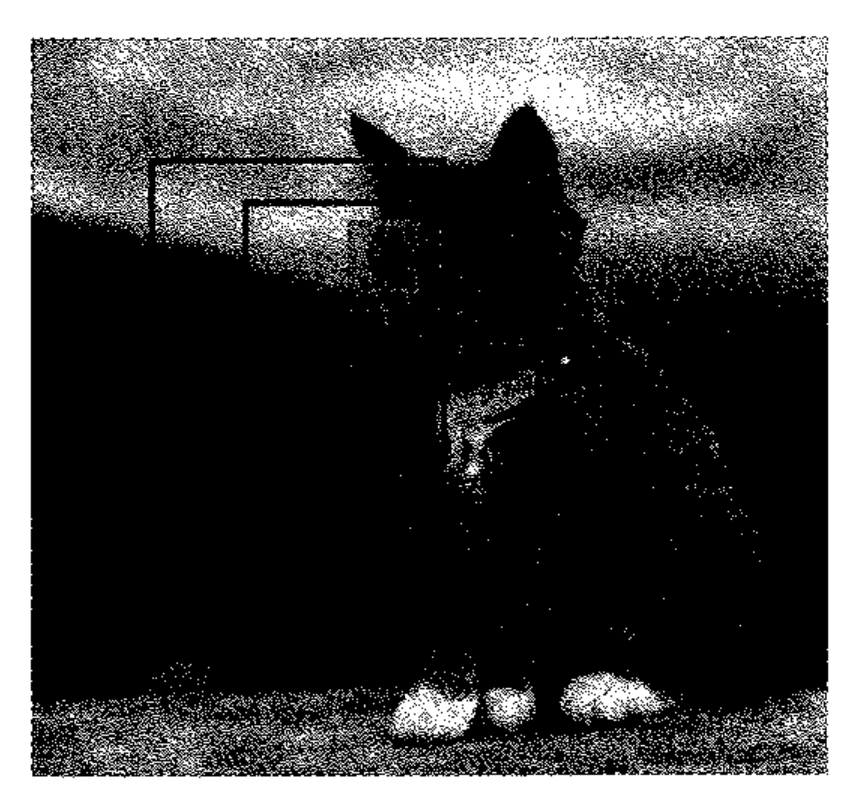
\includegraphics[width=0.42\textwidth]{ch10-fig10-21-滑动窗口冗余.png}
  \caption{当用 CNN 处理来自滑动输入窗口的数据时，出现重复计算的示意图。其中红色框和蓝色框显示了有部分位置重叠的两个输入窗口。绿色框表示第一卷积层中隐藏单元感受野的位置之一，对应隐藏单元激活的计算在这两个窗口位置可以共享。}
  \label{figure:ch10-滑动窗口冗余}
\end{figure}

\begin{figure}[htbp]
  \centering
  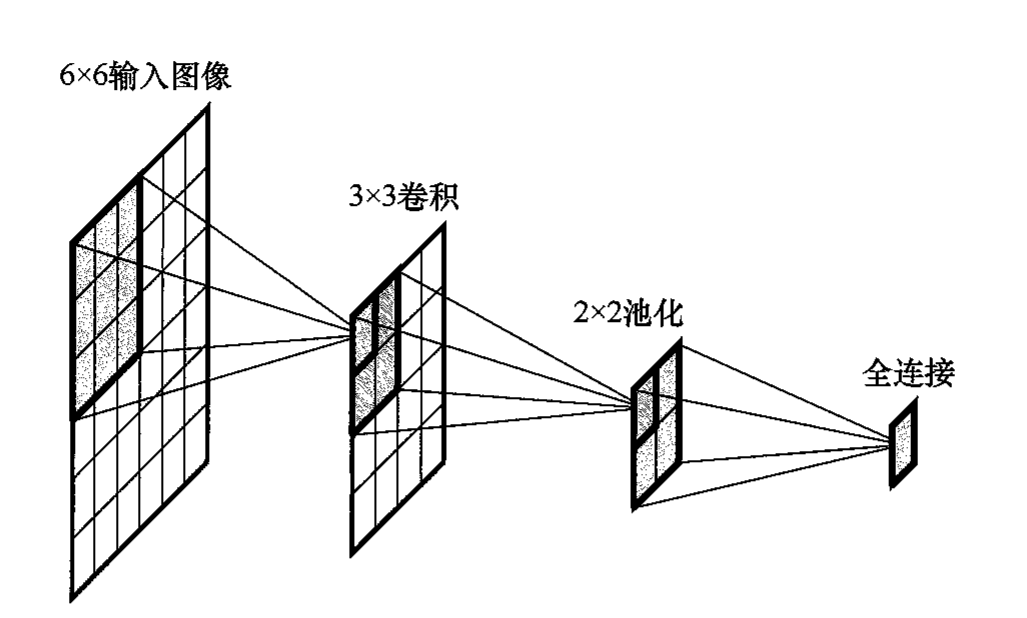
\includegraphics[width=0.6\textwidth]{ch10-fig10-22-简单卷积网络.png}
  \caption{每层具有单通道的简单卷积网络的示例，用以说明用于目标检测的滑动窗口的概念。}
  \label{figure:ch10-简单卷积网络}
\end{figure}

假设该网络是在对象的中心图像上训练的，然后应用于 $8\times 8$ 大小的更大图像，如\cref{figure:ch10-扩展网络}所示。其中，我们只是通过增大卷积层和最大池化层来扩大网络。现在，卷积层的大小为 $6\times 6$，池化层的大小为 $3\times 3$，有 4 个输出单元，每个输出单元都有自己的 softmax 函数。输入其中一个输出单元的权重将在这 4 个输出单元之间共享。我们看到，处理位于输入图像左上角的窗口位置所需的计算与处理训练阶段原始 $6\times 6$ 输入的计算相同。对于其余的窗口位置，则只需要少量的额外计算，如蓝色方块所示。与简单地重复应用完整卷积网络相比，这显著提高了效率（见\cref{exercise:ch10-12}）。注意，现在全连接层本身具有卷积结构。

\begin{figure}[htbp]
  \centering
  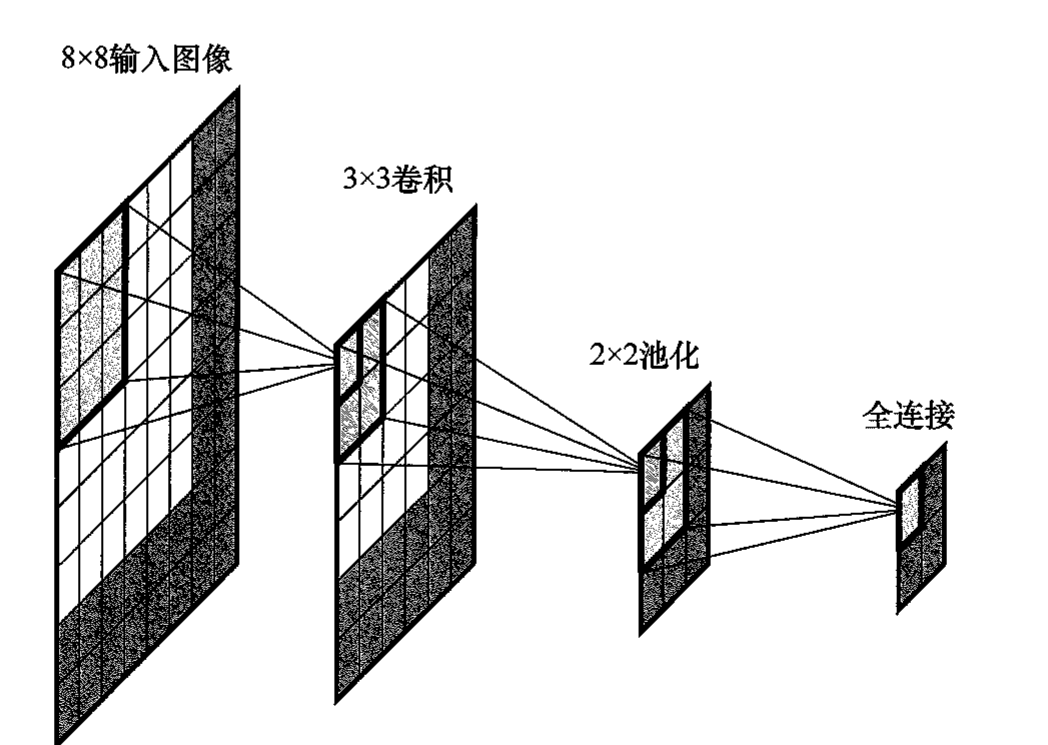
\includegraphics[width=0.6\textwidth]{ch10-fig10-23-扩展网络.png}
  \caption{将\cref{figure:ch10-简单卷积网络}所示的简单卷积网络应用于较大的图像，所需的额外计算对应于蓝色区域。}
  \label{figure:ch10-扩展网络}
\end{figure}

\subsection{跨尺度检测}\label{subsection:ch10-跨尺度检测}

除了在图像中寻找不同位置的对象之外，还需要在不同尺度和不同的宽高比下寻找对象。例如，猫直立时为其绘制的边界框，与其躺下时为其绘制的边界框具有不同的宽高比。与使用输入窗口具有不同大小和形状的多个检测器相比，使用固定输入窗口并制作多个具有不同水平和垂直缩放因子的输入图像副本的方式更加简单，但是效果相同。后者在每个图像副本上扫描输入窗口以检测对象，并使用关联的缩放因子将边界框坐标转换回原始图像空间，如\cref{figure:ch10-多尺度检测}所示。

\begin{figure}[htbp]
  \centering
  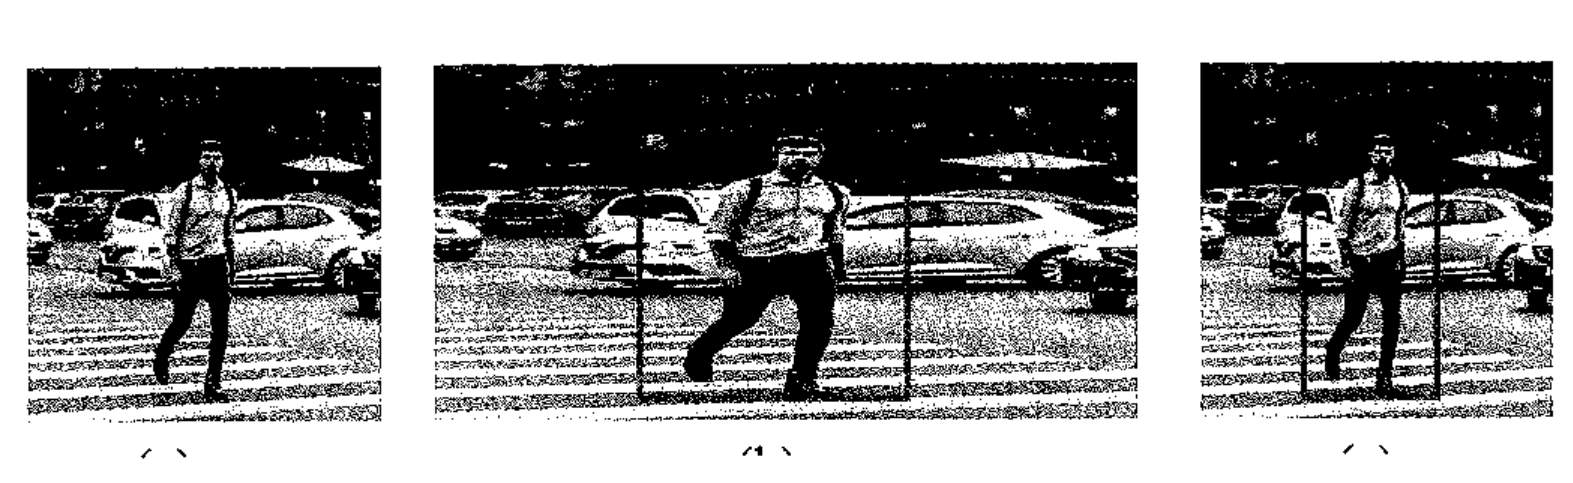
\includegraphics[width=0.8\textwidth]{ch10-fig10-24-多尺度检测.png}
  \caption{使用固定输入窗口在多个尺度和宽高比下检测和定位对象的示意图。原始图像 (a) 被复制多次，并且每个副本在水平和/或垂直方向上被缩放，如 (b) 中的水平缩放所示。然后在缩放的图像上以固定大小的窗口进行扫描。当以高概率检测到对象时，如 (b) 中的红框所示，可以将相应的窗口坐标投影回原始图像空间，从而确定相应的边界框，如 (c) 中所示。}
  \label{figure:ch10-多尺度检测}
\end{figure}

\subsection{非最大抑制}\label{subsection:ch10-非最大抑制}

通过在图像上扫描训练好的卷积网络，可以检测图像中同一类别对象的多个实例，以及来自其他类别对象的实例。然而，这也倾向于在相似位置产生同一对象的多个检测结果，如\cref{figure:ch10-非最大抑制}所示。可以使用非最大抑制（non-max suppression）来解决这个问题，对于每个对象类别，非最大抑制的工作方式如下：首先在整个图像上运行滑动窗口，并计算每个位置存在该对象类别的概率；然后消除所有概率低于某个阈值（例如 $0.7$）的边界框，得到类似于\cref{figure:ch10-非最大抑制}所示的结果——具有最高概率的框被认为是有效检测，并且将相应的边界框记录作为预测结果；接下来，将任何与有效检测的边界框的 IoU 超过某个阈值（例如 $0.5$）的其他框丢弃，从而消除针对同一对象的多个邻近检测结果；最后在剩余的框中，将具有最高概率的框选为另一个有效检测，并且重复上述消除步骤。将这个过程持续下去，直至所有边界框要么丢弃，要么选为有效检测。

\begin{definition}[非最大抑制]\label{definition:ch10-非最大抑制}
给定同一类别的一组候选边界框及其得分（例如属于该类别的概率），以及得分阈值 $p$ 与重合阈值 $\iota$，\textbf{非最大抑制}（non-max suppression）按如下步骤给出保留集合 $\mathcal{K}$：
\begin{enumerate}
  \item 丢弃所有得分低于 $p$ 的候选框；
  \item 在剩余框中取得分最高者 $B^\ast$，将其加入 $\mathcal{K}$ 并从候选集中删除；
  \item 删除候选集中所有与 $B^\ast$ 的 IoU 超过 $\iota$ 的框；
  \item 重复第 2、3 步，直至候选集为空。
\end{enumerate}
\end{definition}

% SUPPLEMENT: parent=definition:ch10-非最大抑制; kind=motivation; location=紧随其后的 remark（重构新增）
\begin{remark}（重构新增）
非最大抑制处理的是滑动窗口方法的固有冗余：同一对象会被多个位置、多个尺度同时检出，且这些框高度重合。算法用两个阈值把两类错误分开：$p$ 控制“要不要这个检测”（低于 $p$ 的直接丢弃，减少假阳性），$\iota$ 控制“两个检测是否指同一对象”（IoU 高则视为重复）。两个阈值的作用不同，不能合并：把 $\iota$ 调大可以保留密集排列的不同对象（如人群），把 $\iota$ 调小则更激进地合并。定义对每个类别独立执行，因为不同类别的框可以合法地重合。算法必然终止：每一步至少删除一个框，候选集有限。注意它不保证找到全局最优的框组合，只是一个贪心过程。
\end{remark}

\begin{figure}[htbp]
  \centering
  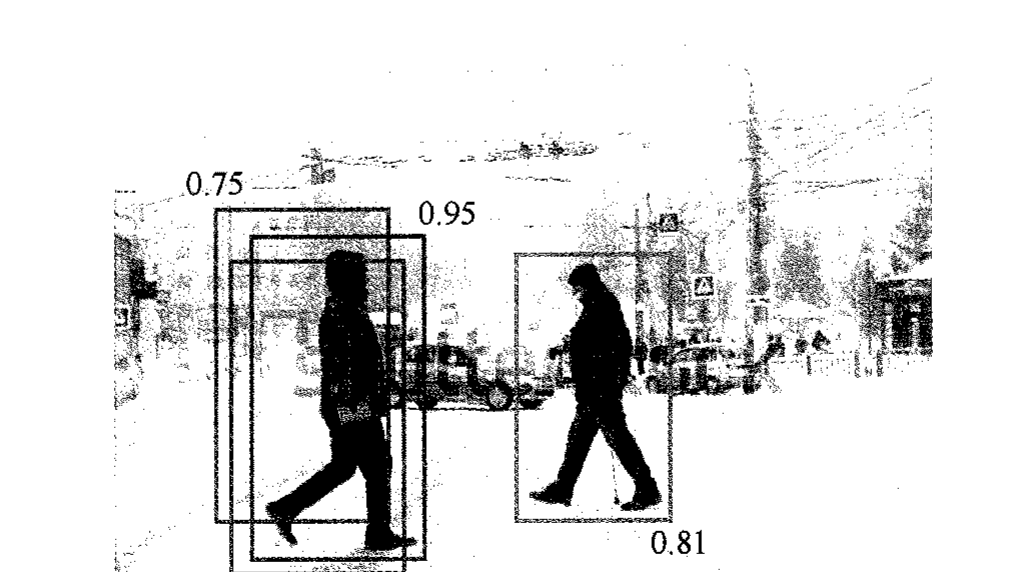
\includegraphics[width=0.6\textwidth]{ch10-fig10-25-非最大抑制.png}
  \caption{同一对象在临近位置被多次检测及关联概率的示意图。红色边界框对应于最高的总体概率。非最大抑制消除了以蓝色显示的其他重合候选边界框，同时保留了以绿色边界框显示的对同一对象类别的另一实例的检测结果。}
  \label{figure:ch10-非最大抑制}
\end{figure}

\subsection{快速区域卷积神经网络}\label{subsection:ch10-快速区域卷积神经网络}

扫描窗口方法将深度卷积网络的全部力量应用于图像的所有区域，即使一些区域不太可能包含对象。另一种方法是应用一些计算成本较低的技术，例如分割算法，来识别图像中存在对象可能性较高的区域，然后仅对这些区域应用完整的卷积网络。这种方法称为带有 CNN 的快速区域提议（fast Region proposals with CNN, fast R-CNN）（Girshick, 2015）。也可以使用区域提议（region proposal）卷积网络来识别最有可能的区域，这种方法称为 faster R-CNN（Ren et al., 2015），该方法允许对区域提议网络和检测定位网络进行端到端训练。

滑动窗口方法的一个缺点是，如果想要非常精确地定位对象，则需要考虑大量的只有细微间隔的窗口位置，这将使计算成本变得很高。一种更高效的方法是将滑动窗口与直接边界框预测结合起来（Sermanet et al., 2013）。在这种情况下，可以连续输出预测边界框相对于窗口位置的位置，以便对预测位置进行一些微调。

\begin{definition}[区域提议]\label{definition:ch10-区域提议}
称一个低成本的预处理过程为\textbf{区域提议}（region proposal），若它从图像中给出少量候选区域，使得真实对象以高概率落在其中，从而可以把昂贵的分类与定位网络只作用于这些区域。若提议过程本身由一个卷积网络实现并与检测网络联合训练，则称相应的检测框架为 \textbf{faster R-CNN}；若提议由外部算法给出、只对区域做分类与框回归，则称 \textbf{fast R-CNN}。
\end{definition}

% SUPPLEMENT: parent=definition:ch10-区域提议; kind=motivation; location=紧随其后的 remark（重构新增）
\begin{remark}（重构新增）
区域提议的要点是“用便宜的计算换掉昂贵的穷举”：滑动窗口对所有位置一视同仁，而区域提议先用颜色、边缘或浅层特征排除明显不含对象的区域。定义区分 fast 与 faster 的关键在于提议是否可学习：前者把提议当作固定输入，检测网络无法通过提议的错误反向传播；后者把提议网络也纳入训练，两个网络共享特征，因此可以端到端优化。这不是命名上的细节，而是训练目标是否一致的问题：提议与检测若分开训练，二者的召回率与定位精度可能相互错配。
\end{remark}

\end{document}
